\documentclass[12pt]{report}
\usepackage{graphicx}
\usepackage[utf8]{inputenc}
\usepackage[spanish]{babel}
\usepackage{setspace}
\usepackage{geometry}
\usepackage{titlesec}
\usepackage{times}
\usepackage{mathptmx} % Use mathptmx instead of times
\usepackage{fancyhdr}
\usepackage{float}
\usepackage{pdfpages}



% Configuración de márgenes
\geometry{
    top=2.5cm,
    left=3cm,
    right=3cm,
    bottom=2.5cm
}

% Configuración de interlineado
\onehalfspacing

% Configuración de títulos y subtítulos
\titleformat{\chapter}[display]
  {\normalfont\bfseries\centering}{}{0pt}{\fontsize{14}{16}\selectfont}
\titleformat{\section}
  {\normalfont\bfseries}{\thesection}{1em}{\fontsize{12}{14}\selectfont}
\titleformat{\subsection}
  {\normalfont\bfseries}{\thesubsection}{1em}{\fontsize{12}{14}\selectfont}


% Configuración de pie de página
  \fancyhf{}
\fancyfoot[R]{\thepage}
\pagestyle{fancy}
\fancypagestyle{plain}{
  \fancyhf{}
  \fancyfoot[R]{\thepage}
}

  \begin{document}
  \pagenumbering{roman}
%----- PORTADA ----
\setlength{\hoffset}{27 pt} % 1 (Para centrar más la portada)
\begin{titlepage}
{\centering
{\fontfamily{ptm}\scshape\bfseries\fontsize{29.16}{34.992}\selectfont Universidad de Guadalajara \par}
\vspace{0.5cm}
{\scshape\Large Centro Universitario de los Lagos \par}
\vspace{1cm}
{\scshape\Large División de Estudios de la Biodiversidad e innovación Tecnológica \par}
\vspace{1cm}
{\graphicspath{{imagenes/Portada}} %ruta de las imagenes

\includegraphics[width=0.3\textwidth]{image.png}\par}
\vspace{1cm}
% Título
{\scshape\large\bfseries Practica 2: CIRCUITO DE AUTOENERGIZACIÓN
DOMINANTE ON Y DOMINANTE OFF \par}
\vspace{0.5cm}
% Materia
{\large \textbf{Materia:} \\Controladores Lógicos Programables\par}
\vfill
% Estudiante
{\large \textbf{Presenta:} \\Oscar Iván Moreno Gutiérrez \#220942754
\\Maximiliano Frias Campos \#217488066
\par}
\vfill
% Profesor
{\large \textbf{Profesor:} \\Dr. Afanador Delgado Samuel Mardoqueo \par}
\vfill
\vfill
% Fecha
\begin{flushright}
  {\normalsize \textbf {Fecha:} \\ \today}
\end{flushright}
\vfill}
{\large  \par}
\end{titlepage}
%----- FIN DE PORTADA ----

%----- ÍNDICE GENERAL ----
\tableofcontents
\newpage

%----- PALABRAS CLAVE ----
\pagenumbering{arabic}
\chapter*{Palabras Clave}
\addcontentsline{toc}{chapter}{Palabras Clave}
\begin{itemize}
  \item PLC: Controlador Lógico Programable.
  \item Autoenergización: Circuito de retención o memoria.
  \item Dominante ON: Circuito que enciende la carga al presionar Arranque y Paro simultáneamente.
  \item Dominante OFF: Circuito que apaga la carga al presionar Arranque y Paro simultáneamente.
  \item Bobina: Componente que controla el relevador o contactor.
  \item Paro: Botón utilizado para detener el circuito.
  \item Arranque: Botón utilizado para iniciar el circuito.
\end{itemize}
\newpage

%----- OBJETIVO ----
\chapter*{Objetivo}
\addcontentsline{toc}{chapter}{Objetivo}
Comprender el funcionamiento del circuito de autoenergización y diferencia entre aquel que es dominante OFF y el que se define como dominante ON.
\newpage

%----- CONTENIDO ----
\chapter{Contenido}
\section{Que es un circuito de autoenergización?}
Un circuito de autoenergización es un circuito de retención o memoria, que se convierte en un circuito básico para todo automatismo. Además, puede implementarse en dos versiones distintas: dominante OFF y dominante ON.

\subsection{Dominante ON}
Cuando se dispone el botón de Paro en serie con el contacto de retroalimentación, el circuito, aunque mantiene su función primordial de autorretención, difiere en la prueba de dominancia, resultando ser del tipo ON, porque al pulsar Arranque y Paro al mismo tiempo, la carga se enciende (Ver figura \ref{fig:dominante_on}).
\begin{figure}[H]
    \centering
    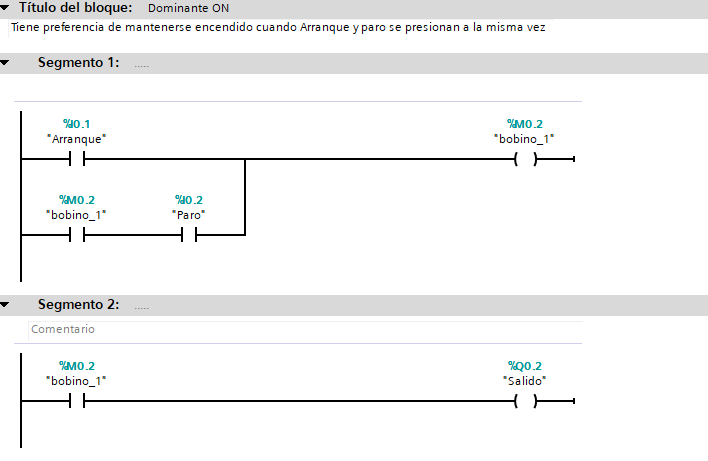
\includegraphics[width=0.5\textwidth]{screenshots/Dominato ON.png}
    \caption{Circuito de autoenergización dominante ON}
    \label{fig:dominante_on}
\end{figure}
\subsection{Dominate OFF}
Se caracteriza por tener el botón de paro en la línea principal que alimenta la bobina del relevador o contactor que controla a la carga. La prueba para identificarlo como dominante OFF consiste en pulsar simultáneamente los botones de Arranque y Paro y observar si la carga permanece apagada. (Ver figura \ref{fig:dominante_off})
\begin{figure}[H]
    \centering
    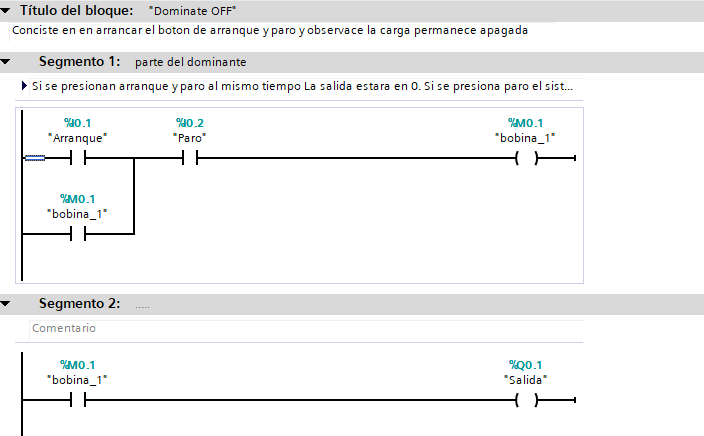
\includegraphics[width=0.5\textwidth]{screenshots/Dominante OFF.png}
    \caption{Circuito de autoenergización dominante OFF}
    \label{fig:dominante_off}
\end{figure}

\section{Materiales}
Para la realización de esta práctica se utilizaron los siguientes materiales:

\begin{itemize}
  \item \textbf{Aplicación con picosoft:} Software utilizado para la simulación y programación de PLCs.
  \item \textbf{PLC:} Controlador Lógico Programable utilizado para la implementación del circuito.
  \item \textbf{Botonera:} Dispositivo que contiene los botones de arranque y paro.
  \item \textbf{Botones:} Componentes individuales de la botonera utilizados para controlar el circuito.
\end{itemize}

\section{Procedimiento}
Creamos un circuito de autoenergización dominante ON y otro dominante OFF en la aplicación Picologo, simulamos el circuito y verificamos su correcto funcionamiento.
Primero Creamos las variables de entrada y salida: (Ambas se usan Para dominante ON y dominante OFF)

\begin{figure}[H]
  \centering
  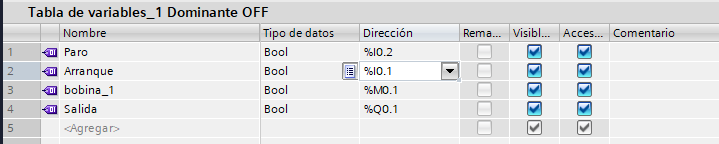
\includegraphics[width=\textwidth]{screenshots/Variables.png}
  \caption{variables de entrada y salida}
  \label{fig:first_image}
  \vspace{1cm} % Optional: Add some vertical space between the images
  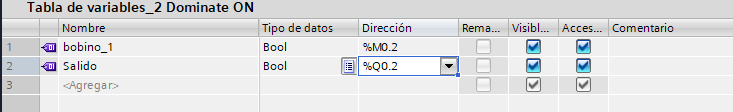
\includegraphics[width=\textwidth]{screenshots/Variables_ON.png}
  \caption{variables de entrada y salida para dominante ON}
  \label{fig:second_image}
\end{figure}

Despues creamos el circuito de autoenergización dominante ON:
\begin{center}

  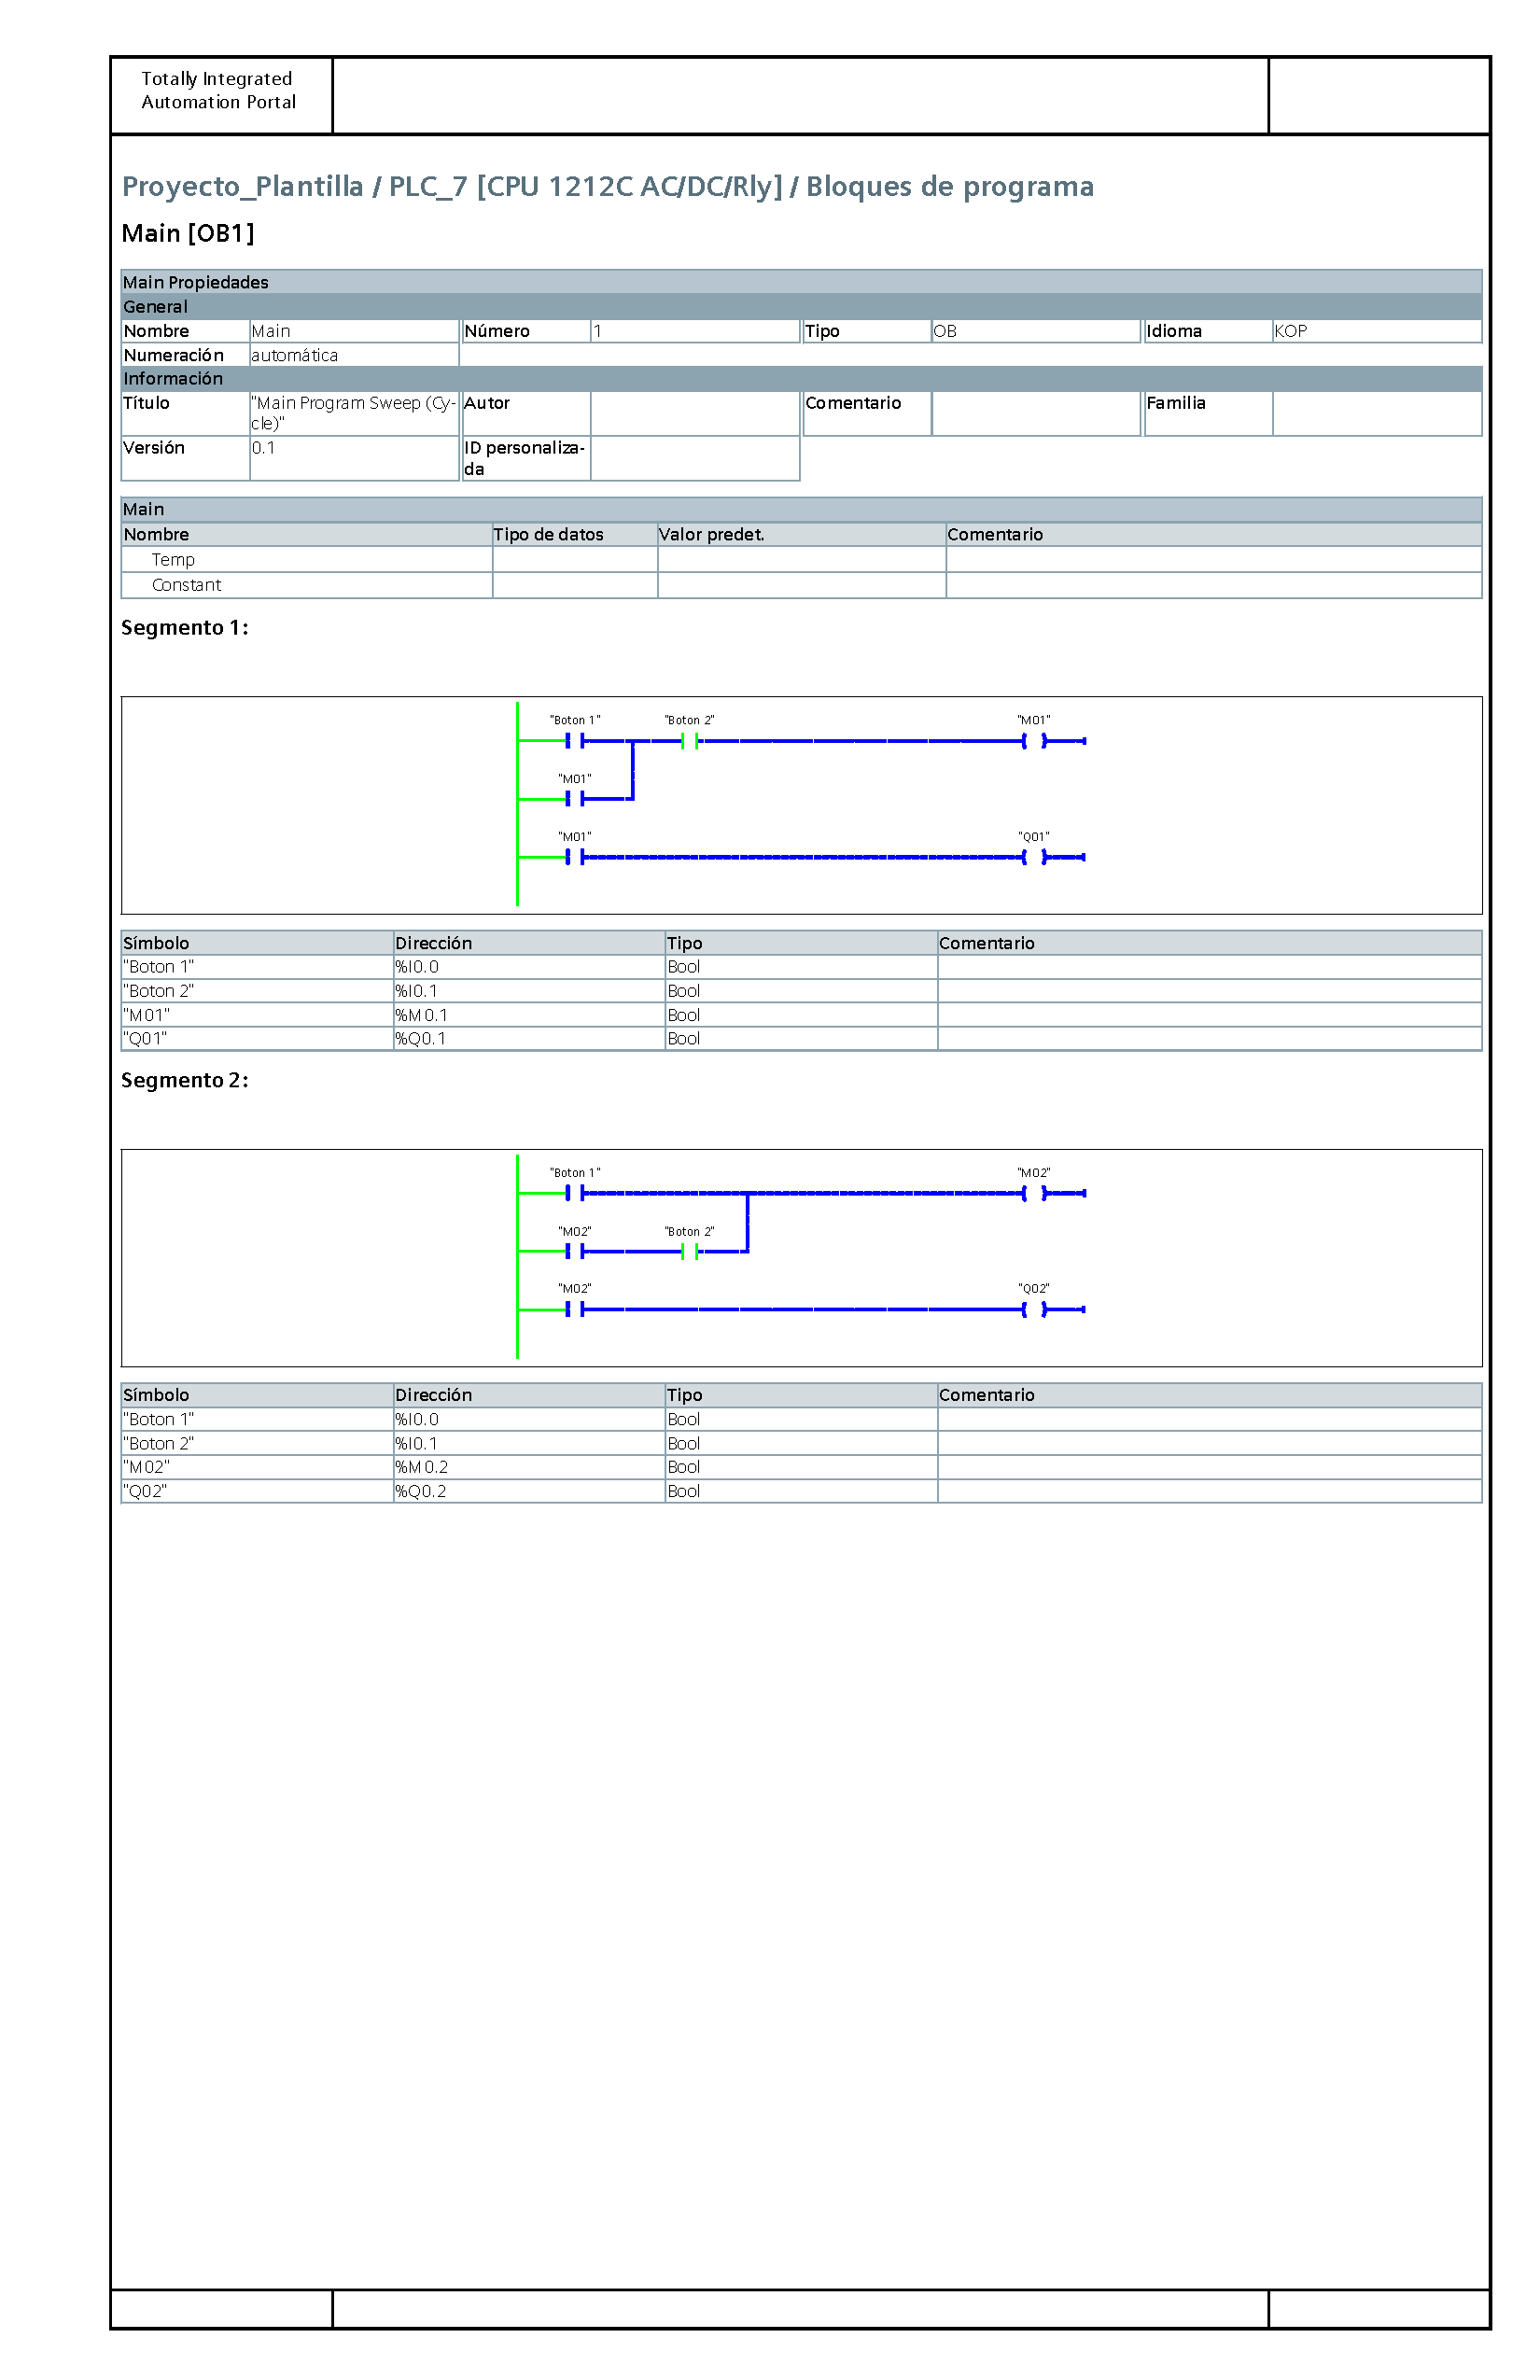
\includepdf[scale=0.9]{screenshots/Practica 2 PLC_Ele.pdf}
\end{center}

Observamos cuando utlizamos el circuito de autoenergización dominante ON, al presionar el boton de arranque y el de paro al mismo tiempo, la carga se enciende. (Vease la figura \ref{fig:dominante_on_output})
\begin{figure}[H]
  \centering
  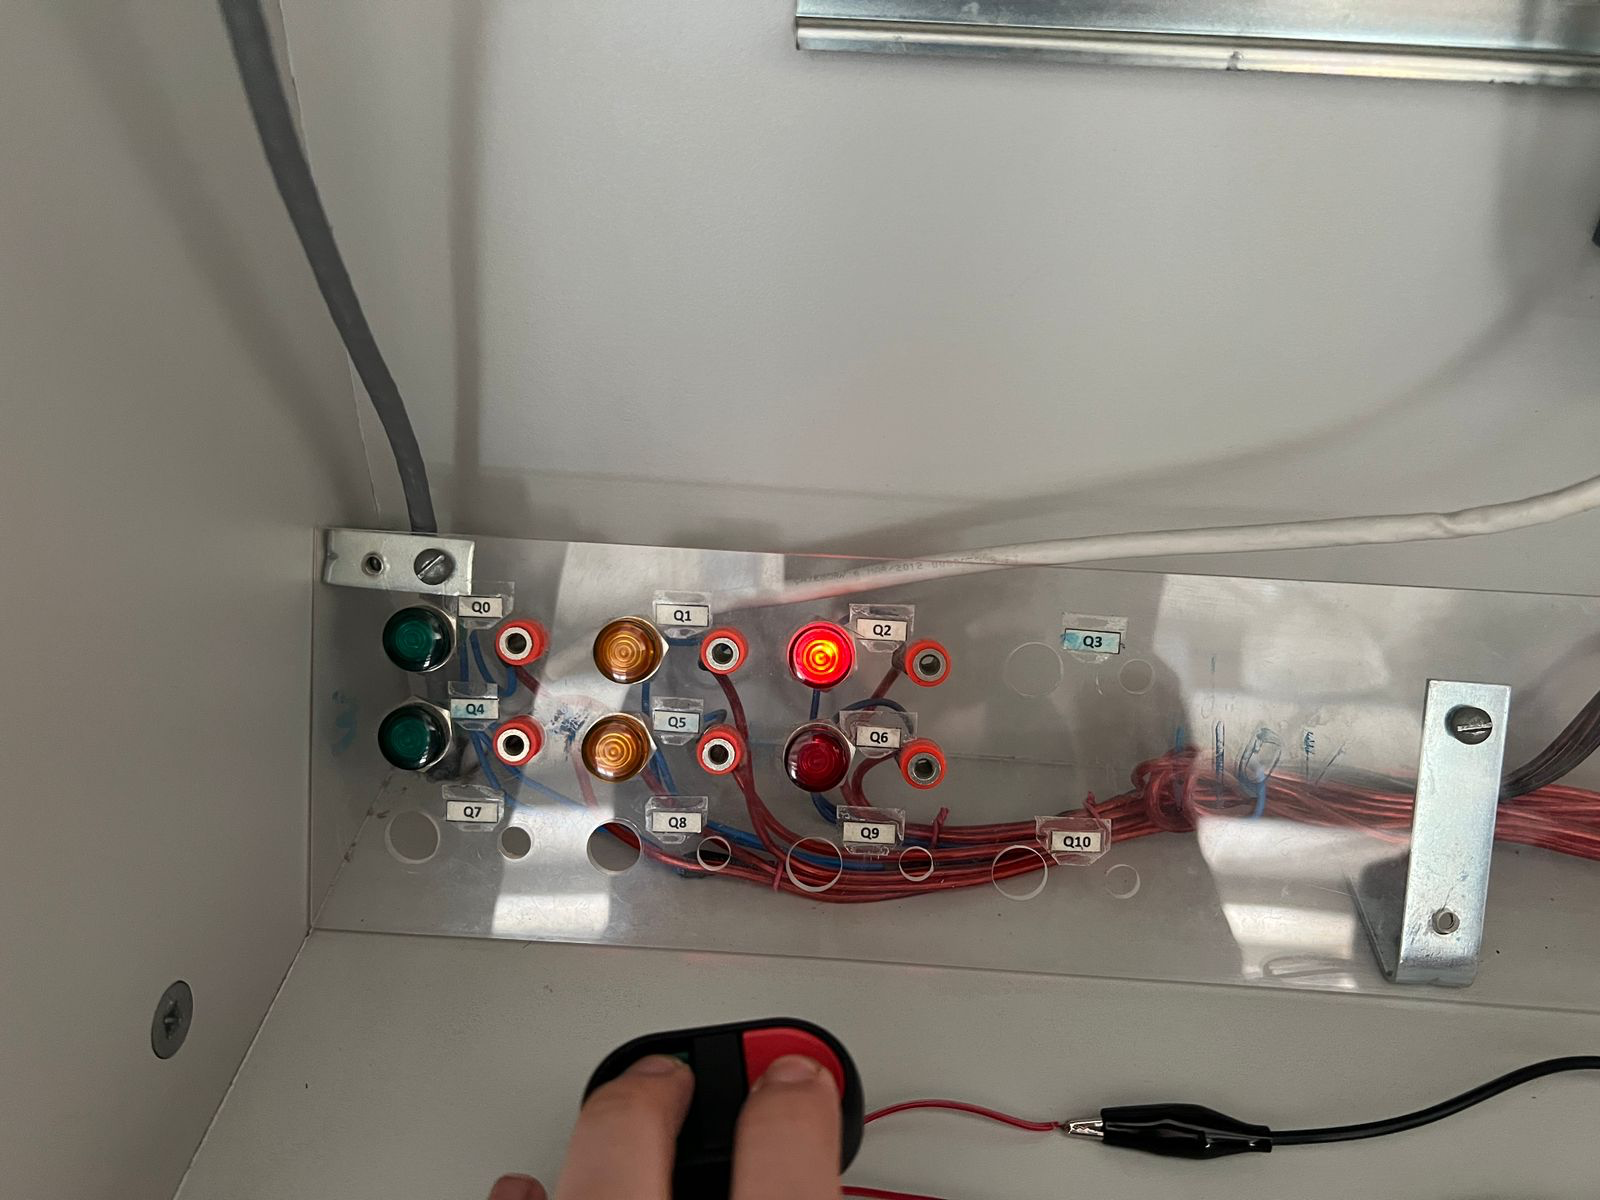
\includegraphics[width=0.5\textwidth]{screenshots/salida_dominante_ON.png}
  \caption{Salida del circuito de autoenergización dominante ON}
  \label{fig:dominante_on_output}

\end{figure}

Y para el circuito de autoenergización dominante OFF, al presionar el boton de arranque y el de paro al mismo, tiempo, la carga se apaga. (Vease la figura \ref{fig:dominante_off_output})
\begin{figure}[H]
  \centering
  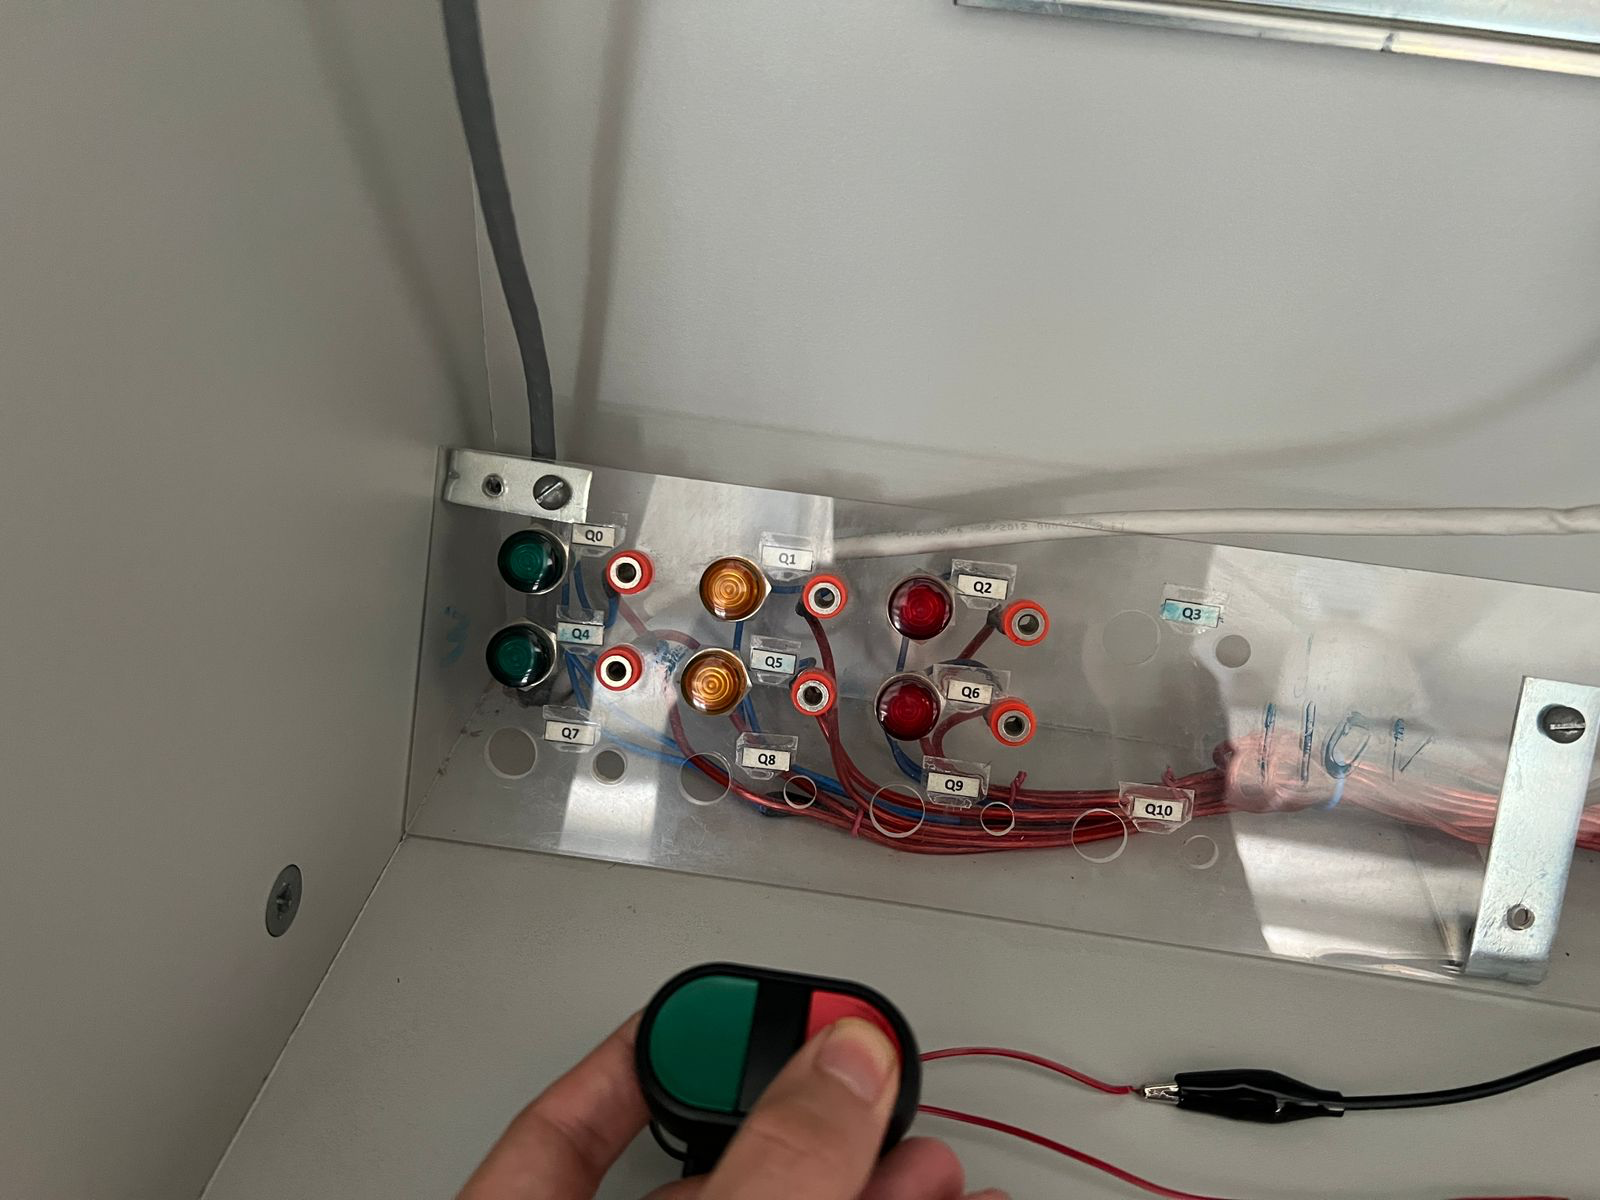
\includegraphics[width=0.5\textwidth]{screenshots/salida_dominante_OFF.png}
  \caption{Salida del circuito de autoenergización dominante OFF}
  \label{fig:dominante_off_output}
\end{figure}
\newpage

%----- CONCLUSIONES ----
\chapter{Conclusiones}
En esta práctica, se logró implementar y simular circuitos de autoenergización dominante ON y dominante OFF utilizando el software Picologo. A través de la creación de variables de entrada y salida, así como la configuración adecuada de los componentes del circuito, se pudo verificar el correcto funcionamiento de ambos circuitos.

El circuito de autoenergización dominante ON demostró ser efectivo al mantener la carga encendida incluso después de soltar el botón de arranque, mientras que el circuito de autoenergización dominante OFF permitió apagar la carga al presionar simultáneamente los botones de arranque y paro.

Estos resultados son fundamentales para comprender el comportamiento de los circuitos de autoenergización y su aplicación en sistemas de control industrial. La práctica proporcionó una experiencia valiosa en la programación y simulación de PLCs, así como en la interpretación de los resultados obtenidos.

En conclusión, la práctica no solo permitió afianzar los conocimientos teóricos sobre los circuitos de autoenergización, sino que también brindó una oportunidad para desarrollar habilidades prácticas en el uso de herramientas de simulación y programación de PLCs.
\newpage


\end{document}